\chapter{The \rnn{} Algorithm}%
\label{sec:neuralringer}

This section describes the \rnn{} concepts and the resulting algorithm used for Run~2
operation. Considerations about data sets (Section~\ref{ssec:dataset}) and the \TnP method
(Section~\ref{ssec:tnp}) employed to extract signal and background samples
from real ATLAS data start this section. Section~\ref{ssec:rnn_for_online_and_eletrons} refers to the
decisions made for the \rnn{} development in order to optimize its contributions in saving processing resources. Aiming at better exploring the discriminative
power of ring sums for electron triggers (Section~\ref{ssec:ringer_id}),
an ensemble of neural-networks is employed. Its training procedure and how trigger decisions are made are covered in Section~\ref{sec:tuning}.




\section{Data sets and Event Selection}%
\label{ssec:dataset}

The training procedure for 2017 operation was built with samples of 2015 simulated $Z\rightarrow ee$ decay selected by the $Z\rightarrow ee$ \TnP method (see Section~\ref{ssec:tnp}). Background samples for electron processes were simulated. A filter was applied to enrich the sample in electron backgrounds selecting events where have particles produced in the hard scatter with a summed transverse energy exceeding 17 GeV in a region of $\Delta\eta\times\Delta\phi=0.1\times0.1$. Here, both simulated data offer a pile-up of 60 interactions, average values, per bunch crossing which has never been seen before in collision data until that time (e.g. for 2016 the pile-up peak reached was 40 interactions per bunch crossing.).

After the training stage, the decision is taken by applying a threshold. To set the correct value without cause any inefficiency in the end of the HLT, in data, it was used the full \textit{pp} collision data set recorded by ATLAS in 2016 with LHC operating at a centre-of-mass energy of $\sqrt{s}=13 \text{TeV}$ during of Run 2. The electrons\footnote{To train and evaluate the models it was used the probe electron from the $Z\rightarrow ee$ \TnP method.} was selected by $Z\rightarrow ee$ \TnP method and the offline tight\footnote{The offline \textit{lhtight} criteria.} criteria. For background, it was used objects rejected by the $Z\rightarrow ee$ \TnP method (that does not belong to any tag-probe electron pair) and reproved by the loosest offline available criteria\footnote{The offline \textit{lhloose} criteria for 2016 data and the offline \textit{lhvloose} (very loose) for 2017 and 2018 data.}. For the 2018 operation, the purely data-driven strategy was used, selecting events from the 2017 recorded data to train the models and adjust all thresholds.

The tuning and analysis performed on data recorded between by ATLAS have their quality ensured\footnote{The ATLAS data quality is provide through a strict Data Quality Policy that validates each part of a run data set that can be used for analysis, rejecting any piece affected by a potential underlying inactive of dysfunctional part of the detector.}. To facilitate (big) data manipulation, events of potential interest are derived using specific requirements providing potential \Zee{} \tnp{} candidates and background electrons. 

%
\begin{table}[ht!]%\footnotesize
\centering
\caption{Event selection for tuning the models and defining the discriminant
requirements of the \rnn operating in the Run 2. Symbol ``\veto'' is used to
indicate that the physics object is considered when it is rejected by the
criterion. The label `mc15' corresponds to simulated data based on Monte Carlo
algorithms and `Tier0' correspond to ATLAS experimental
data \cite{aad2020performance}.}\label{tab:event_selection}
% TODO Explain why not loose and not Zee
\resizebox{\textwidth}{!}{%
\begin{tabular}{lp{6.8cm}cc}
\hline \hline
Type & Dataset & \TnP & Offline Selection \\
\hline \hline
\multicolumn{4}{c}{2017 Models} \\
\hline
signal &
mc15\_13TeV.361106.PowhegPythia8EvtGen\allowbreak{}\_AZNLOCTEQ6L1\_Zee.merge.AOD.\allowbreak{}e3601\_s2876\_r7917\_r7676
& \Zee & None \\
background &
mc15\_13TeV.423300.Pythia8EvtGen\allowbreak{}\_A14NNPDF23LO\_perf\_JF17.merge.AOD.\allowbreak{}e3848\_s2876\_r7917\_r7676
& None & None \\
\hline
\multicolumn{4}{c}{2017 Discriminant Requirements} \\
\hline
signal & 2016 Tier0 + EGAM1 (p3013) + GRL v88 & \Zee & \tight \\
background & 2016 Tier0 + EGAM7 (p3013) + GRL v88 & \veto\Zee & \veto\loose \\
\hline
\multicolumn{4}{c}{2018 Models and Discriminant Requirements} \\
\hline
signal & 2017 Tier0 + EGAM1 (p3336) + GRL v97 & \Zee & \tight \\
background & 2017 Tier0 + EGAM7 (p3336) + GRL v97 & \veto\Zee & \veto\vloose \\
\hline \hline
\end{tabular}
}
\end{table}




\subsection{\TnP Method}\label{ssec:tnp}

The \tnp{} method relies on the existence of resonances that decay to a pair of particle of interest (\Zee{}, \Jee{}, $\gamma \rightarrow ee$ and etc) ~\cite{PERF-2016-01}. In the case of electrons coming from $Z$ boson decays, the selection of two EM objects with a mass around the $Z$ mass with opposite charge is enough to get a pure sample of electrons as soon you tag one of those objects as a well identified electron. The remaining object can them be assumed to be an electron with a very high underlying purity. This object can them be used as a probe to test the electron trigger efficiency. The selection of the tag particle is done according to offline analysis criteria to make sure that the trigger selection introduces a minimal loss of those events at the final physics analysis level~\cite{aaboud2019electron}. A single electron is used to select the event at the trigger level (tag), allowing the second electron to be used as a probe to measure trigger algorithm performance~\cite{aad2020performance}.


\section{Algorithm Development}\label{ssec:rnn_for_online_and_eletrons}

The \rnn{} algorithm was initially proposed for electron-jet discrimination. 
During Run 2, both online and offline versions
were considered for  development, but the scarcity of available human resources restricted the scope of developments, which focused on reducing CPU demands of the online electron triggers. Within the electron triggers, \hlt{} selection is
specially relevant to single object triggers, which, in turn, use the most of the trigger bandwidth~\cite{aad2020performance}. Particularly, the primary single electron triggers
are currently evaluated and developed using \Zee{} \tnp{} samples 
(Section~\ref{ssec:tnp}), in which most electrons have $\et>\SI{15}{\GeV}$, which is the region of interest in physics studies and on which the \rnn{} developments focus. The result of this effort
follows.


\subsection{Building the Rings}\label{top:algorithm}

The ATLAS calorimeters comprise rectangular cells in the
\etaphi axis\footnote{Except for the forward calorimeters.}. Thus, an actual conic structure cannot be defined
without intensive processing of the cell energy information. As the algorithm was
considered to operate online, approximations were  made. Especially, the rectangular structure of
the rings follows the instrumentation and the ring coverage is bounded to the RoI area. In addition, the granularity changes from the cell sizes (e.g., barrel to end-cap) are neglected in order to employ a
grid-like algorithm.


Here, the algorithm RoI covers a
region of the calorimeter, centered in the L1 provided RoI, of
$0.4\times0.4$ in the $\eta\times\phi$ plane. The algorithm
starts on the second EM sampling layer (EM2)\footnote{This convention is used for all sampling layers, thus HAD1 stands for the first hadronic layer, HAD2 the second hadronic layer etc.}, where position (given in $\eta\times\phi$ plane) of the cell with
highest $E_T$ on the algorithm RoI is taken as the center of the cascade
interaction with the calorimeter. The initial seed cell position is propagated to other calorimeter layers in order to define the axis of the rings in that layer. Then, for each layer, the algorithm refine the seed position searching for the hottest cell inside of the window centered by the EM2 initial seed. The refined seed ($c_{hot,l}$) will be used as start point to build the rings. A ring $R_{n,l}$ contains all cells in calorimeter layer $l$ which are $n$ cells from the refined seed (See Figure~\ref{fig:building_rings_a} for an illustration of the parameters). Formally,


\begin{equation}
%\label{eq:ring_idx}
R_{n,l} = \left\{c_{n,l} \mid n = \left\lfloor \max{\left( 
\frac{| \eta_{i,l} - \eta_{hot,l} |}{h_{\eta,l}}, 
\frac{| \phi_{i,l} - \phi_{hot,l} |}{h_{\phi,l}} 
\right)} \right\rceil, 
\forall c_{i,l} \in
\Theta_{RoI,l}
\right\},
\end{equation}



\noindent where (analogous to $\phi$ when suitable): $\eta_{i,l}$
and $\eta_{hot,l}$ are respectively the $c_{i,l}$ and $c_{hot,l}$
cells position in $\eta$; $h_{\eta,l}$ is the $l^{th}$ layer cell size in $\eta$; $\Theta_{RoI,l}$ is the set of cells
in the $l^{th}$ layer which are within the Ringer RoI.
\tablename~\ref{tab:ring_alg_parameters} shows the number rings computed at each layer and the respective granularity.


\begin{table}[ht!]
\centering
\caption{Nomenclature defining the ringer algorithm layers and sections, as well
  as the respective parameters employed and calorimeter sampling
  layers from which the cells are extracted. The ringer algorithm
  parameters are dependent on the ringer layer $l$ and independent on \eta{} and
  \et{} during Run~2. The parameters are the ring size in \eta{}
  ($h_{\etaa,l}$), $\phi$ ($h_{\phii,l}$) and the number of rings to be computed
  in each layer ($\text{N}_l$). The values for $h_{\etaa,l}$ and $h_{\phii,l}$
  are approximated, the exact ones can be obtained for $\eta=0$ in
  Table~\ref{tab:granularity}.
%To refer to a ring, it will be used notation XYYY, where X is the ring index in
%the YYY layer.
}%
\label{tab:ring_alg_parameters}
\resizebox{.8\textwidth}{!}{%
\begin{tabular}{lc|ccc|ccc}
\hline
\hline
\multicolumn{2}{c|}{Ringer} & \multicolumn{3}{c|}{Calorimeter Sampling} & 
\multicolumn{3}{c}{Parameters} \\
\hline
Section & Layer ($l$) & Barrel & \itc & End-cap & $h_{\etaa,l}$ & $h_{\phii,l}$ & $N_l$ \\
\hline
\hline
\multirow{4}*{EM} & \ps &  \presamplerb & & \presamplere & 0.025 & 0.1 & 8 \\
\cline{2-5}
& \emi & \emb{1} &  & \emec{1} & 0.003 & 0.1 & 64  \\
\cline{3-5}
& \emii & \emb{2} &  & \emec{2} & 0.025 & 0.025 & 8 \\
\cline{3-5}
& \emiii & \emb{3} &  & \emec{3} & 0.050 & 0.025 & 8 \\
\cline{1-5}
\multirow{6}*{HAD} & \multirow{2}*{\hadi} & \tilebar{0} &
\multirow{2}*{\tilegap{3}} & \multirow{2}*{\hec{0}} & \multirow{2}*{0.1} & \multirow{2}*{0.1} & \multirow{2}*{4} \\
&                     & \tileext{0} &                               &                           \\
\cline{3-5}
& \multirow{2}*{\hadii} & \tilebar{1} & \multirow{2}*{\tilegap{1}} & \hec{1}       & \multirow{2}*{0.1} & \multirow{2}*{0.1} & \multirow{2}*{4} \\
&                   & \tileext{1} &              & \hec{2}  \\
\cline{3-5}
& \multirow{2}*{\hadiii} & \tilebar{2} & \multirow{2}*{\tilegap{2}} & \multirow{2}*{\hec{3}} & \multirow{2}*{0.2} & \multirow{2}*{0.1} & \multirow{2}*{4} \\
&                     & \tileext{2} &                &             \\
\hline
\hline
\end{tabular}
}
\end{table}






If no cell is available for a given ring, the correspondent ring
quantity is set to 0.
The sum of the transverse energies of cells $c_{n,l}$ in the ring $R_{n,l}$ form a vector of discriminating quantities. 
They are ordered outwards and from the
innermost layer of the calorimeter and provided the ring-shaped information 
of the RoI. Figure~\ref{fig:building_rings_b} shows the ring-shaped mean profile differences between electrons and jet particles. The implementation of this algorithm is simple and the actual code
was optimized to be fast (see Section~\ref{top:fastcalo_cpu}). 









%%%% Coloring the comment as blue
\newcommand\mycommfont[1]{\footnotesize\ttfamily\textcolor{blue}{#1}}
\SetCommentSty{mycommfont}
\SetKwInput{KwInput}{Input}                % Set the Input
\SetKwInput{KwOutput}{Output}              % set the Output



\begin{algorithm}[H]

    %\DontPrintSemicolon
  
    \KwInput{$\Theta_{RoI,l}$, $\eta_{cluster}$, $\phi_{cluster}$, $h_{\eta,l}$, $h_{\phi,l}$, $N_{l}$}
    \KwOutput{r}

    r $\leftarrow$ initialize with zeros the ring vector with size $N_{l}$
 
    \tcc{Energy, $\eta$ and $\phi$ from the hottest cell.}
    $E_{hot,l}$, $\eta_{hot,l}$, $\phi_{hot,l}$ = 0

    \tcc{Refine the hottest cell position around the cluster center position.}
    \For{$C_{i,l}$ $\leftarrow$ $\Theta_{RoI,l}$}
    {
        $E_{i,l}$ $\leftarrow$ energy from $C_{i,l}$

        $\eta_{i,l}$ $\leftarrow$ central position in $\eta$ from $C_{i,l}$
        
        $\phi_{i,l}$ $\leftarrow$ central position in $\phi$ from $C_{i,l}$

        \tcc{Check if the current cell ($C_{i,l}$) is inside of a window with $0.4\times0.4$.}
        \If{ $(\eta_{cluster}-0.2)$ > $\eta_{i,l}$ e $\eta_{i,l}$ < $(\eta_{cluster}+0.2)$}
        {
            \If{ $(\phi_{cluster}-0.2)$ > $\phi_{i,l}$ e $\phi_{i,l}$ < $(\phi_{cluster}+0.2)$}
            {
                \If{$E_{i,l} > E_{hot,l}$}
                {
                    $E_{hot,l}$ $\leftarrow$ $E_{i,l}$

                    $\eta_{hot,l}$ $\leftarrow$ $\eta_{i,l}$
                    
                    $\phi_{hot,l}$ $\leftarrow$ $\phi_{i,l}$
                }
            }
        }
    }


    \tcc{Fill the energy of each ring using the hottest cell position as the center.}
    \For{$C_{i,l}$ $\leftarrow$ $\Theta_{RoI,l}$}
    {

        $\eta_{i,l}$ $\leftarrow$ central position in $\eta$ from $C_{i,l}$
        
        $\phi_{i,l}$ $\leftarrow$ central position in $\phi$ from $C_{i,l}$

        $\delta_{\eta}$ = $(\eta_{i,l}-\eta_{hot,l})/h_{\eta,l}$

        $\delta_{\phi}$ = $(\phi_{i,l}-\phi_{hot,l})/h_{\phi,l}$

        $n = round(max(\delta_{\eta}$, $\delta_{\phi}))$
                
        \If{n $\leq$ $N_{l}-1$}
        {
            $E_{i,l} \, \leftarrow$ energy from $C_{i,l}$

            $r[n] += E_{i,l}$

        }  
    }
    
    \tcc{Calculate the transverse energy for each ring given $\eta_{hot,l}$}
    \For{ i = 0; i < $N_{l}$; i++}
    {
        $r[i] = \frac{r[i]}{\cosh(|\eta_{hot,l}|)}$
    }

  \Return{r}


\caption{Rings build algorithm.}
%\label{alg:ringer_alg}
\end{algorithm}




\begin{figure}[!ht]
  \begin{center}
  \begin{subfigure}[c]{.48\textwidth}
  \centering
  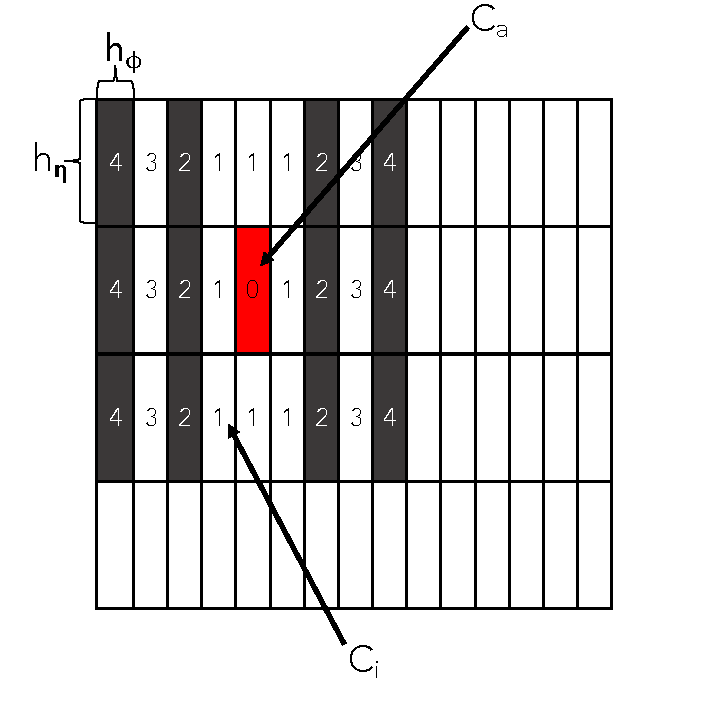
\includegraphics[width=\textwidth]{sections/ringer/figures/reco_steps/ring_em1_mask.pdf}
  \caption{}
  \label{fig:building_rings_a}
  \end{subfigure}\\
  \centering
  
  \begin{subfigure}[c]{.7\textwidth}
  \centering
  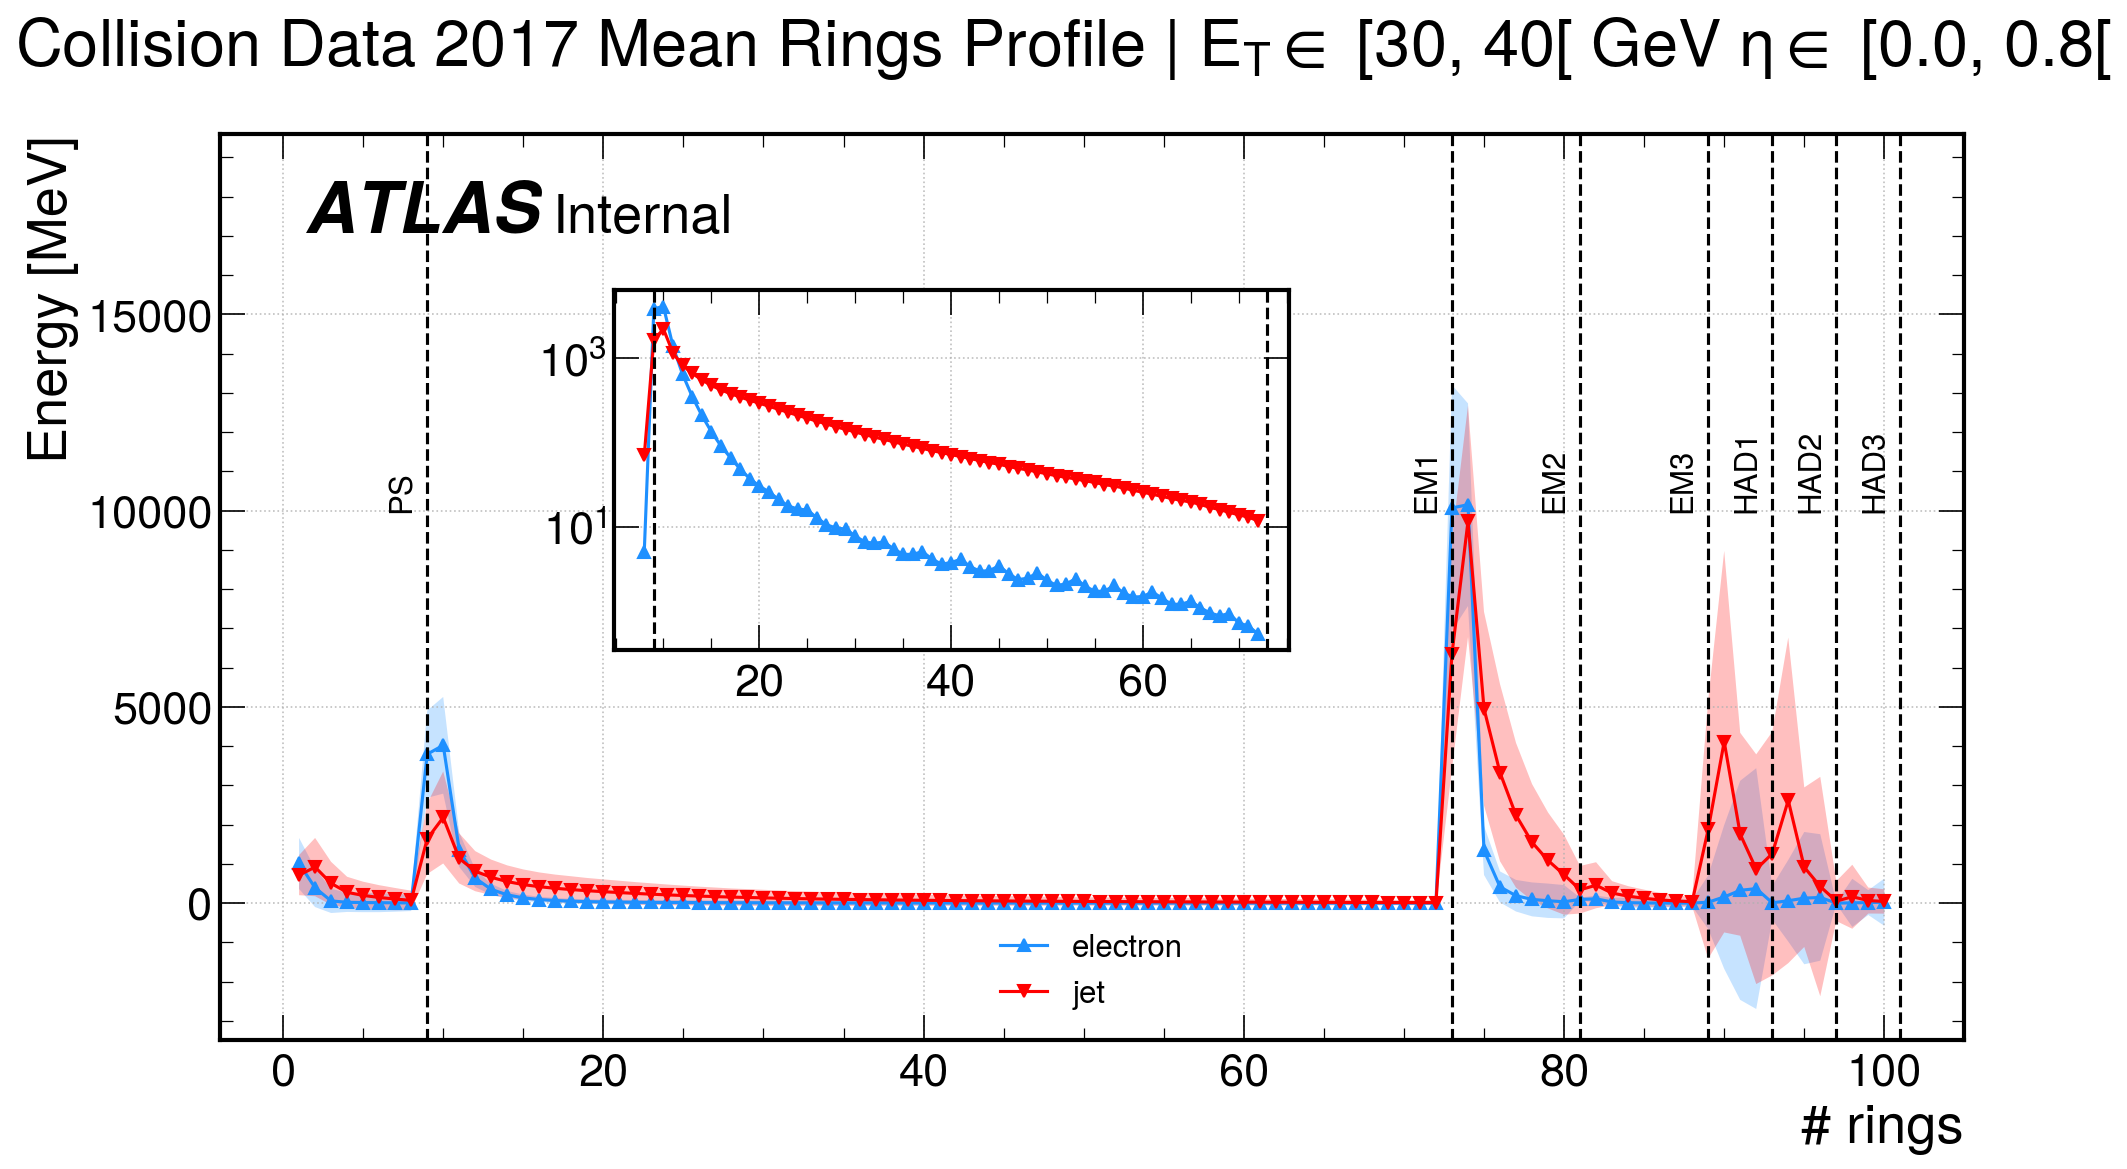
\includegraphics[width=1.1\textwidth]{sections/ringer/figures/reco_steps/data17_zee_mean_rings_profiles_et2_eta0.png}
  \caption{}
  \label{fig:building_rings_b}
  \end{subfigure}
  \caption{
  Top: illustration of the \fastcalo algorithm for building ring sums in the EM1, sketching of the computation of $n$ for the first four rings in a hypothetical layer.
  	Bottom: average rings profile from collision data at $30 \leq E_T < 40$ GeV and $0.0 \leq \eta < 0.8$ for each layer of the calorimeter. The embedded profile shows the EM1 layer rings in a logarithmic scale. Here, it is possible to observe that most part of the energy for the electrons is absorbed by the eletromagnetic layers. For the jets, the opposite is observed and most part of the energy is absorved by the hadronic layers.}
  \end{center}
\end{figure}





\section{Ring Sums as Discriminant Variables}\label{ssec:ringer_id}

% TODO Add references of sucesfull aplications of NNs in other fields.

%The ring sums compose a space with distinct nature with respect to the standard
%shower shape variables, where the first contains higher redundancy between its
%variables. Although the use of univariate cuts or a likelihood model could be
%considered, they have limitations to explore concisely the statistical
%dependency.
To deal with the high redundancy between the ring variables, we benefit from machine learning processing to unveil the latent discriminating space, as in
the case of a Multi-layer Perceptron (MLP) neural-networks~\cite{haykin_2008},
employed for Run~2 operation. 
%MLPs require a normalization preprocessing step~\cite{haykin_2008} to adjust the input dynamic range to the neuron activation function employed (Section~\ref{top:pp}). 
An ensemble of MLPs was employed for operation by tuning and selecting
the models per regions of the \eteta space (Section~\ref{top:nn_ensemble}), whose
motivations are driven by physics, instrumentation and software 
engineering. The \rnn
%engineering. In the same way, \rnn 
decision making is also based on division of the phase space in regions, and the discriminant requirement is
computed as a linear function of \avgmu to pursue signal efficiency invariance
to pile-up contributions. 
The strategy to structure the MLPs,  and train the hyper-parameters of the ensemble and tune of discriminant requirements 
%The strategy, structure of the MLPs and hyper-parameters for training the ensemble and tuning of discriminant requirements 
are described in Section~\ref{sec:tuning}.

%\begin{figure}[h!t]
%\centering
%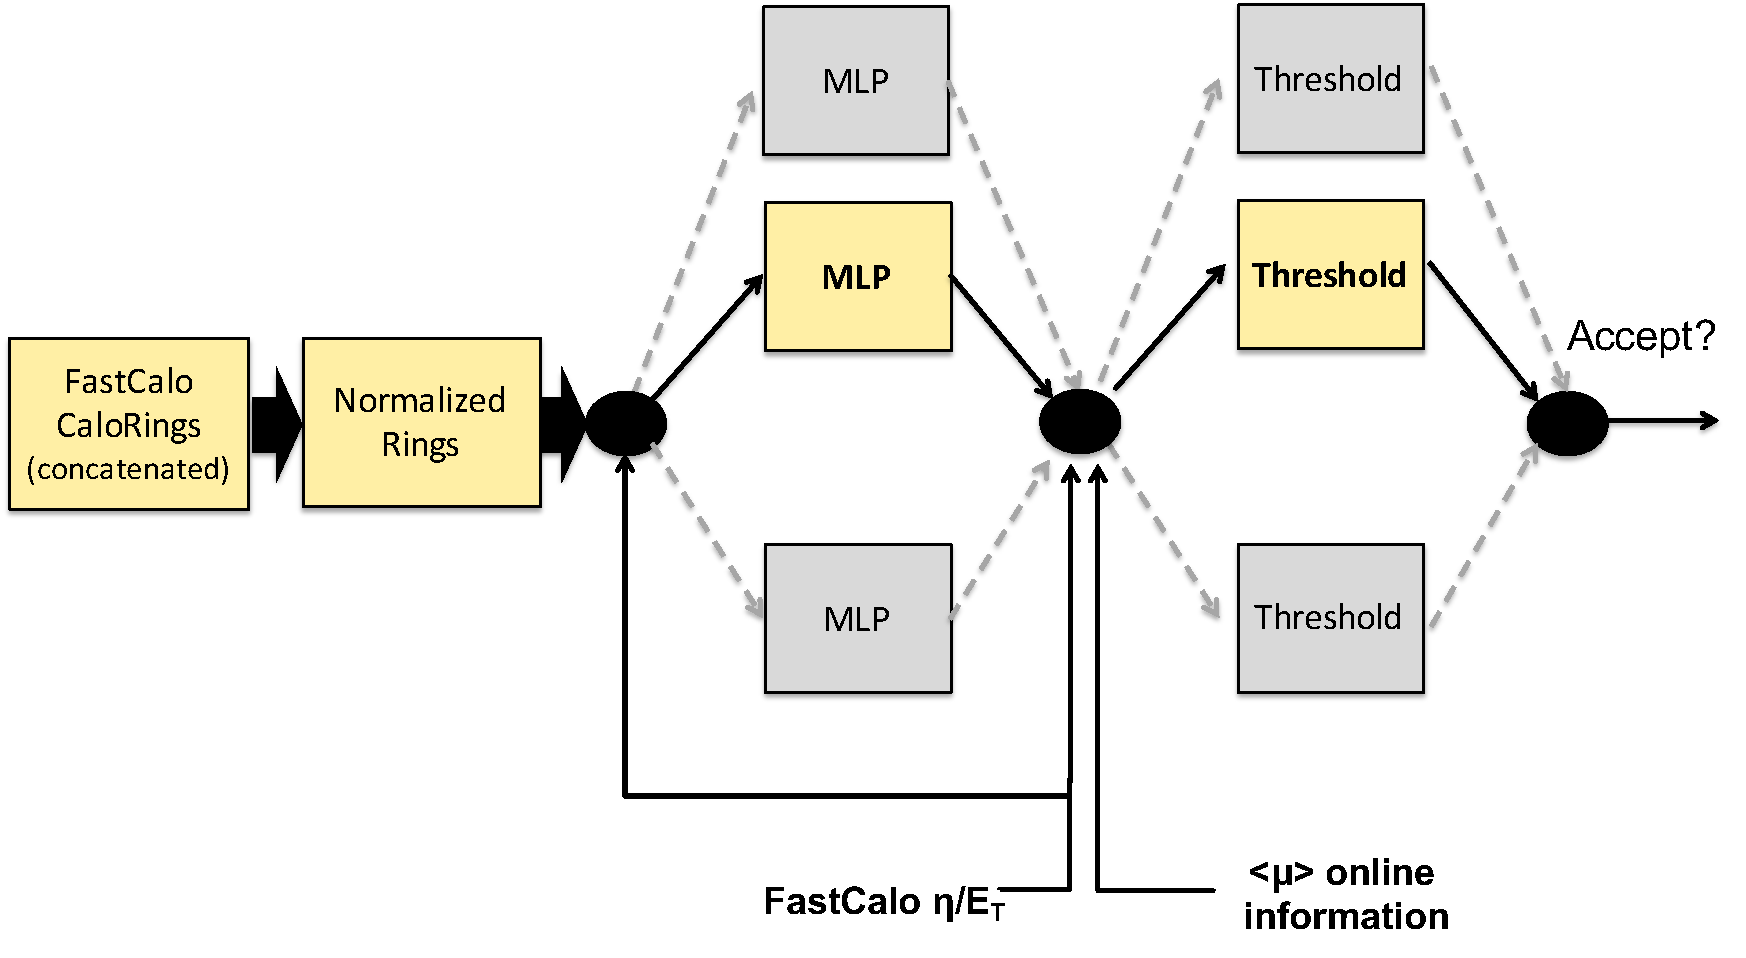
\includegraphics[width=0.9\textwidth]{sections/ringer/figures/Ensemble.pdf}
%\caption{\label{fig:ensemble}
%Processing flow diagram of the \rnn{} ensemble operation and decision making
%during Run~2.
%}
%\end{figure}

%
%%% Coloring the comment as blue
\newcommand\mycommfont[1]{\footnotesize\ttfamily\textcolor{blue}{#1}}
\SetCommentSty{mycommfont}
\SetKwInput{KwInput}{Input}                % Set the Input
\SetKwInput{KwOutput}{Output}              % set the Output



\begin{algorithm}[H]

    \DontPrintSemicolon
  
    \KwInput{Rings, $E_{T}$, $\eta$, \avgmu{}, models, thresholds}
    \KwOutput{Decision}

    Decision = False \tcc{Set the decision to false by default}
 
    \tcc{model is an object with attributes etmin, etmax, etamin, etamax and hold the neural network struture.}

    \For{model \leftarrow models}
    {
        % If et cluster is 
        \If{$E_{T}$ of the cluster is within the $E_{T}$ upper and lower bounds of the model}{
        {
            \If{$|\eta|$ of the cluster is within the $\eta$ upper and lower bounds of the model }
            {
                output $\leftarrow$ Propagate the normalized rings through the neural network and get the output}                
                \textbf{break}
            }

        }
    }
  

    \For{parameters \leftarrow thresholds}
    {
        \If{$E_{T}$ of the cluster is within the $E_{T}$ upper and lower bounds of the parameters }
        {
            \If{$|\eta|$ of the cluster is within the $\eta$ upper and lower bounds of the parameters}
            {
                \tcc{get the slope and offset parameters to apply the pileup corretion}
                \alpha $\leftarrow$ get slope from parameters

                \beta $\leftarrow$ get offset from parameters

                \tcc{check if output is higher than the threshold}
                \If {output > $\alpha\avgmu{}+\beta$}
                {
                    Decision = True \tcc{approve the event.}     
                }

                \textbf{break}
            }
        }
    }



\caption{Ringer ensemble algorithm}
\label{alg:ensemble}
\end{algorithm}


\subsection{Ring Sum Normalization}\label{top:pp}

The current strategy concatenates all rings in a single vector of 100
variables. An absolute normalization using the total RoI energy, as in
(\ref{eq:ring_norm}), is applied to normalise the variables. This procedure was
initially proposed and examined by~\cite{1995_seixas_ringer}, as a way of
preserving the shower energy profile in fractions of the total energy. The
absolute term is used to avoid reflecting the values along the axis due to
negative noise accumulation, a behavior which would impact the physics
representation of the normalized values and require a more complex decision
boundary:

\begin{equation}
  r^\prime_{k} = \frac{r_{k}}{| \sum\limits_{i=1}^{100} r_i
  |}, \;\;\;
    \forall \; k\in\{1,\dots,100\}.
\label{eq:ring_norm}
\end{equation}

A study on simulation data showed that this strategy had compatible
efficiency to other possible normalization schemes. It is specially valuable for its
simplicity (nonparametric approach) and for allowing easy interpretation of the
shower profile. These reasons motivated its usage for Run 2.
%, however this strategy is subject to diminish signal contributions at stringent pile-up
%contamination, specially at low-energy operation due to lower signal-to-noise ratio.  
%Specifically, energy contributions from outer hadronic rings can
%dominate and deteriorate signal profile. We expect to review this strategy for
%Run~3, in particular when considering low-energy triggers ($<\SI{15}{\GeV}$).

\subsection{Motivation for an Ensemble of Neural Networks}\label{top:nn_ensemble}

The normalized concatenated ring vector feeds an ensemble of MLPs. A single
model is drawn from the ensemble for operation based on the nearest (Euclidean
distance) region on the \eteta space for which it was designed.
%In the following, we address the reasons for adopting such an ensemble.

In regards to calorimetry, the usage of an ensemble with specific models per
phase space region allows to mitigate fluctuations in the variable profiles
%(Figure~\ref{fig:ring_distortion}) 
due to the detector response and energy differences of the showers.
%response (Section~\ref{ssec:calo}). %and limitations of the online algorithm
%(Section~\ref{top:algorithm}) 
%in the observed signatures of the physics objects.
A large contribution comes from granularity changes, which are discrete
in the phase space. Other important factors 
influencing such profiles are the
amount of the material as a function of \abseta{} and the dependence of
underlying processes in the shower development with respect to the incoming
particle energy. Although these alterations are mostly continuous, it is also
possible to approach the problem using space discretization.

%Regions overlapping two distinct granularity are not handled by
%this approach. Other sources, as
%the variation in the shower profile due to the energy and amount of material
%(see Figures~\ref{fig:cal_em_x0} and~\ref{fig:cal_had_lambda}), contribute with
%modifications in the variable profiles that may not be completely mitigated with
%hard-bounded regions. Similarly, One additional contribution is
%the pseudorapidity and transverse energy measurements, which are subject to the
%uncertainties of the \fastcalo{} reconstruction.
%as the different shower uniformity~\cite{Wigmans2017}\hspace{0.01\textwidth}

\begin{comment}
\begin{figure}[h!t]
\centering
\begin{subfigure}[c]{.6\textwidth}
\centering
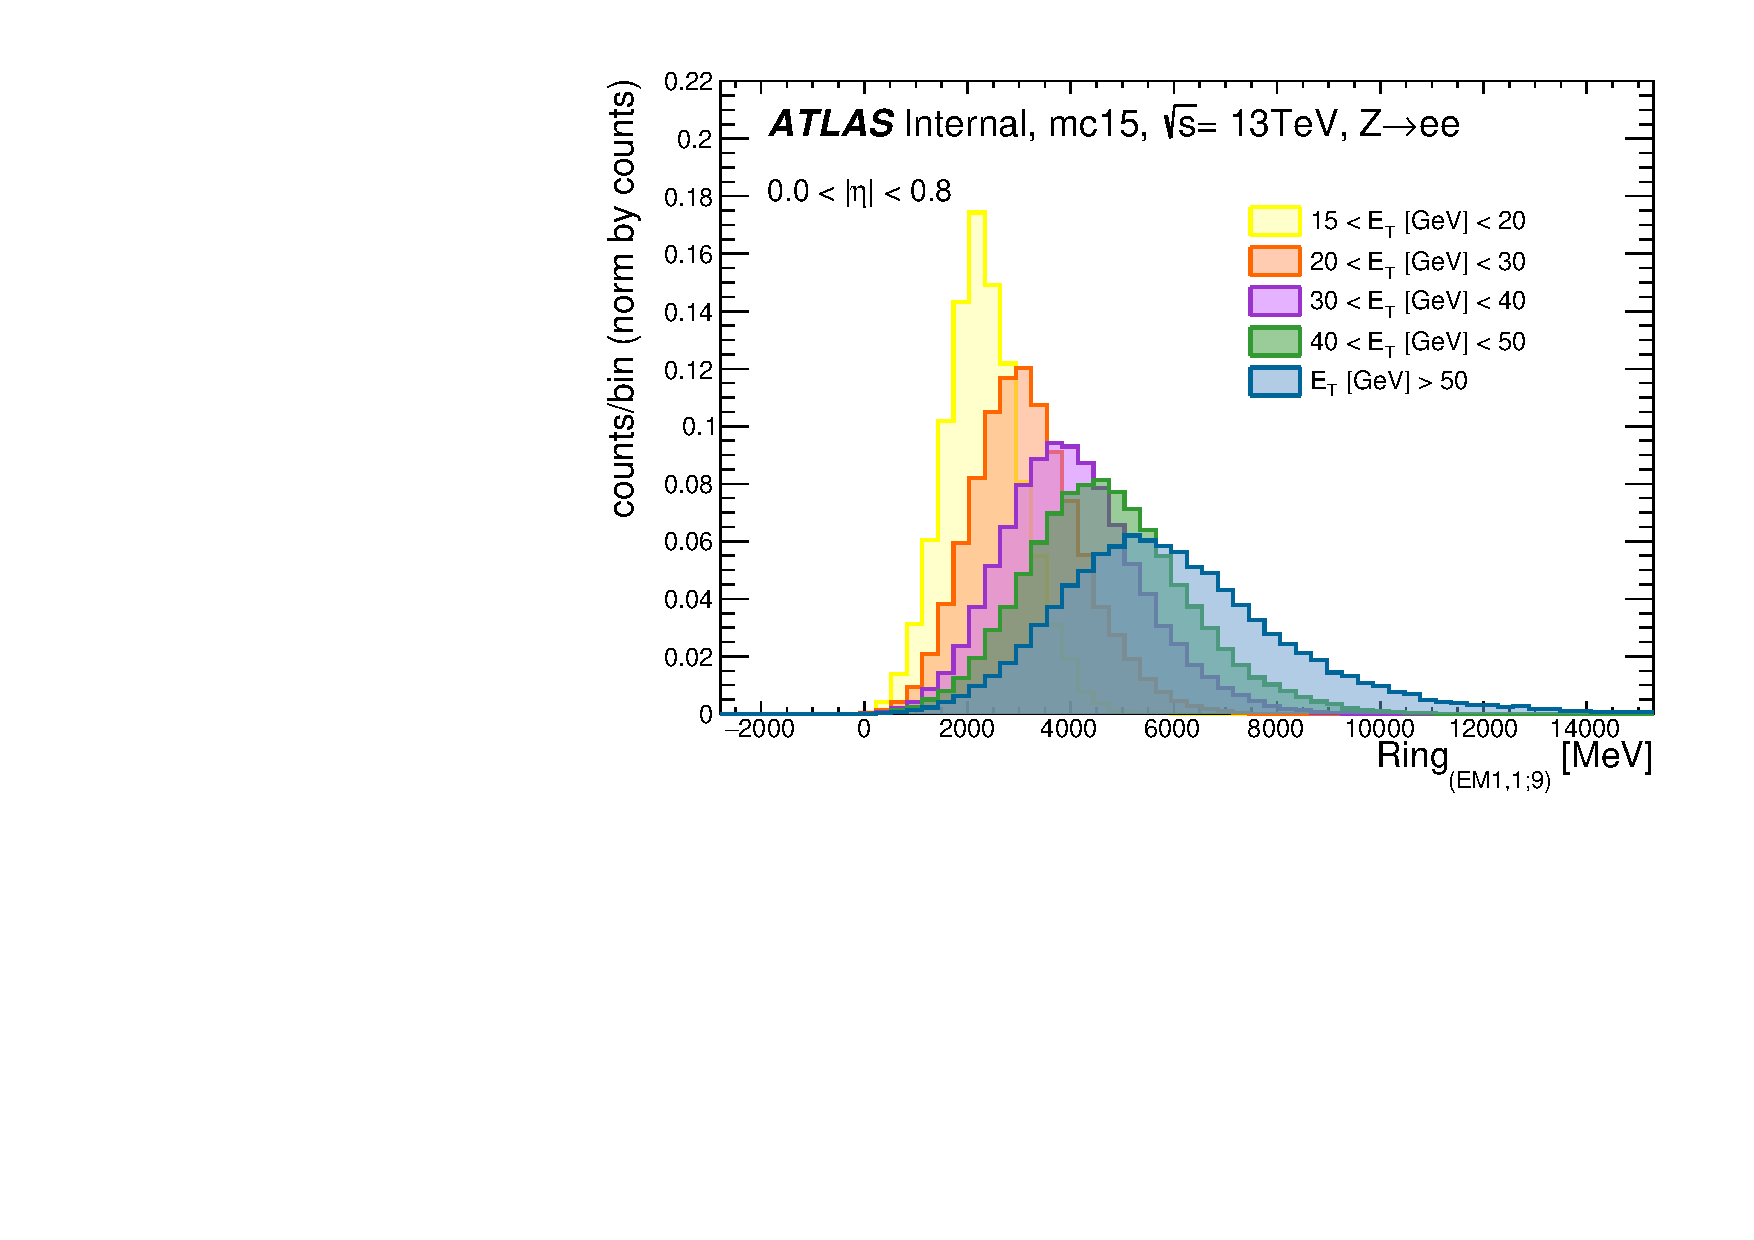
\includegraphics[width=\textwidth]{sections/ringer/figures/L2Calo_ring_9_eta0_etComp.pdf}
\centering
\caption{}%
\end{subfigure} \\
\begin{subfigure}[c]{.6\textwidth}
\centering
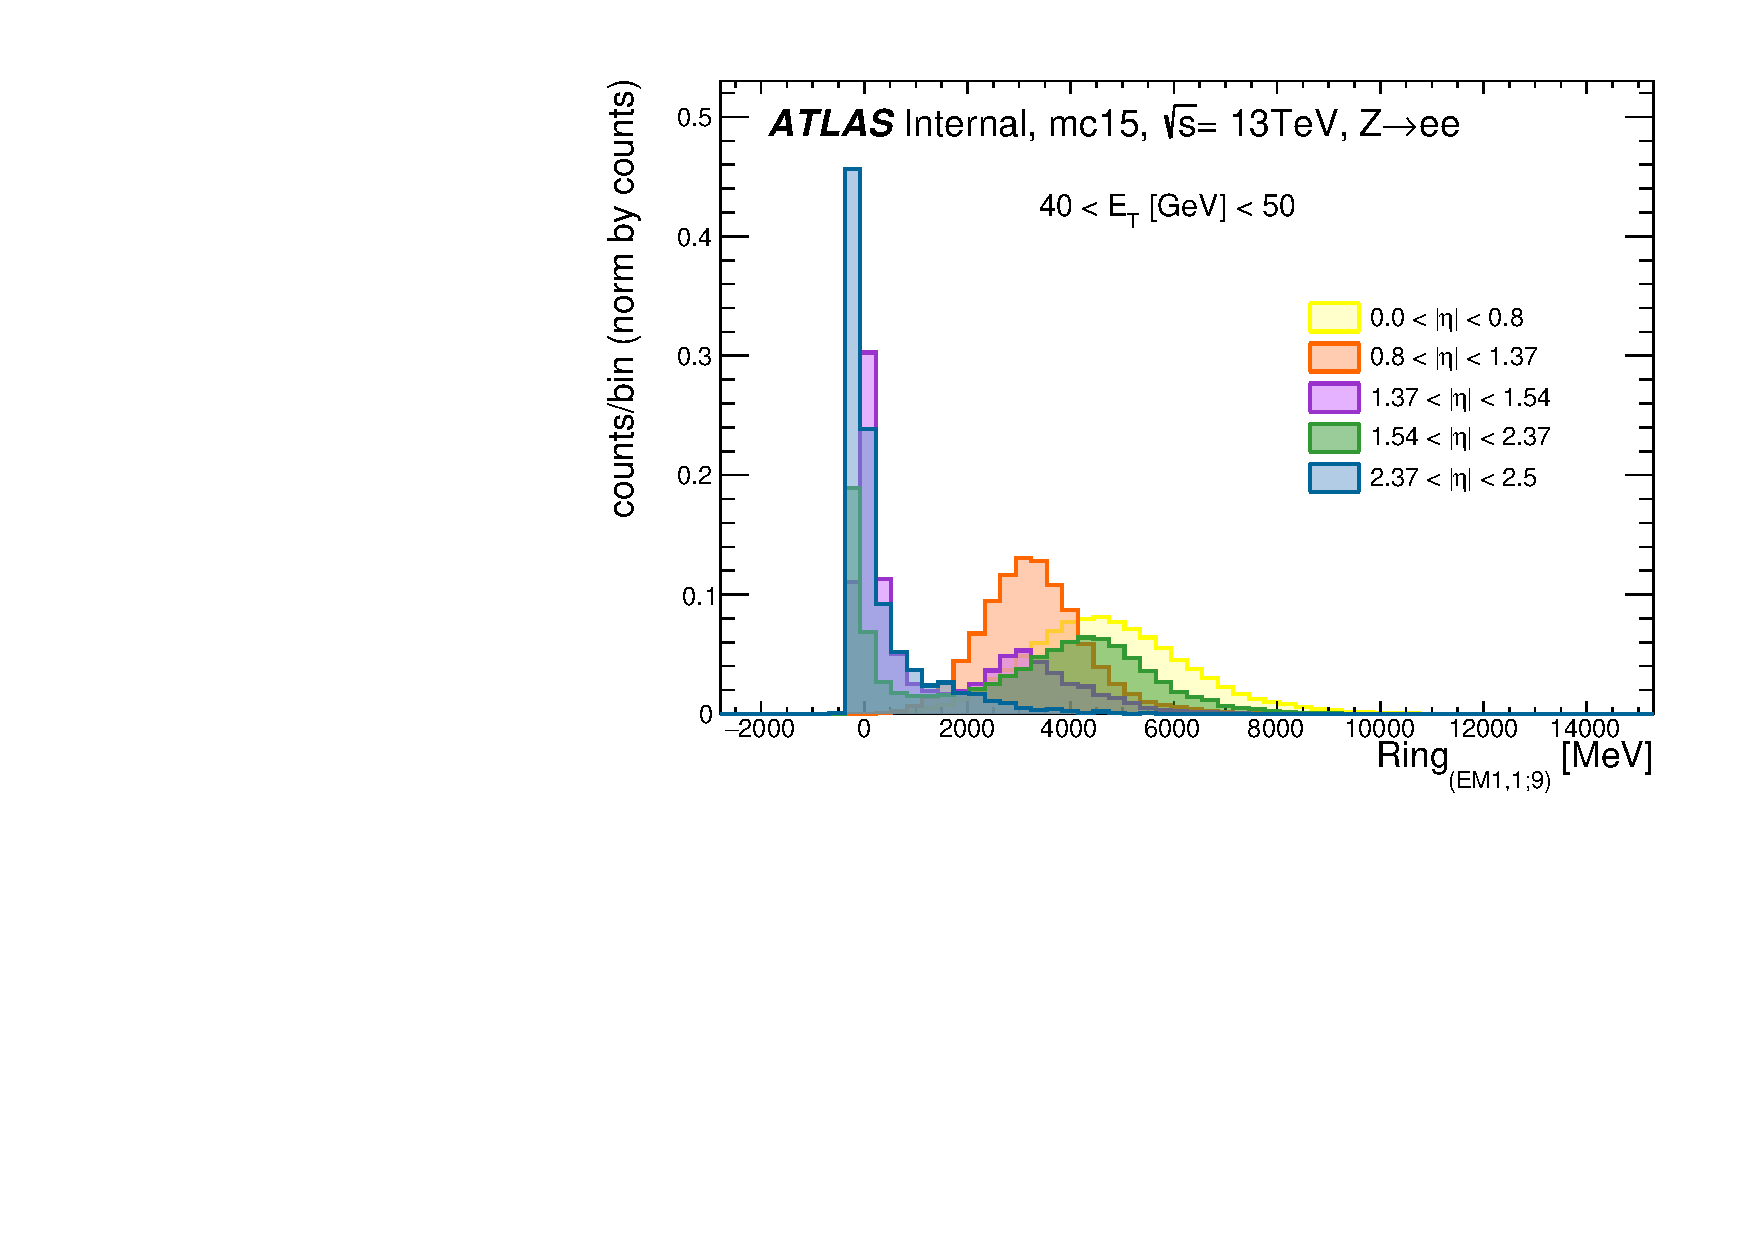
\includegraphics[width=\textwidth]{sections/ringer/figures/L2Calo_ring_9_et3_etaComp.pdf}
\caption{}%
\end{subfigure} 

\caption{Marginal distributions of the non-normalized first ring (hottest cell)
in the EM1 for the \et (a) and  \abseta (b) in Z$\rightarrow$ee simulated data
for the boundaries employed for extracting the \rnn{} discriminants in 2017.}%
%\label{fig:ring_distortion}
\end{figure}
\end{comment} 

In physics, such ensemble approach is consistent with the unfolding
strategy~\cite{Cowan1998}, usually employed for correcting for
measurement distortions due to the limitations of the instrumentation. It relies
on the definition of regions in variable space leading to these
variations (\eteta{}) where the detector efficiency, as well as other
sources of interference, are approximately constant. Once classification
efficiencies are evaluated using regions, it is natural that model parameters
are also defined for these regions. It is the case of the electron likelihood
algorithm~\cite{atlas_electron_id_offline}, which motivated the usage of
\eteta{} regions in the \rnn{} algorithm.

At the software level, the ensemble allows to handle all data in memory at once,
which speeds up the training cycle. Limiting the memory requirement for tuning
the models is particularly interesting in order to benefit from low-memory 
 processing nodes, which were predominantly available in 
WLCG~\cite{2015_lcg_tdr} during our
developments.\@ In addition, the decomposition of the problem can also lead to a
reduction of the training time~\cite{Polikar2006}, as observed heuristically\footnote{
  When using NVIDIA RTX 2080Ti in tensorflow 1.14 and a minibatch size of 1024, a 
  MLP with single hidden layer, we observed a substantial increase in the runtime (from 4 
  to 41 seconds per epoch) with respect to the ensemble version.} when
comparing the tuning time of the ensemble to a single and more complex model.
This effect can be related to the reduction of conflicting training information,
which can occur when a network is forced to learn several dissimilar functions
(as distinct decision boundaries for each region)~\cite{Auda1999,haykin_2008}.
Regarding the operation, the proposed ensemble only requires the choice of a
single model to operate instead of a more often committee machine approaches
that require the computation of different models in parallel with a fusion
method~\cite{zhou_ensemble}.  Therefore, the chosen ensemble configuration adds
minimal overhead in terms of trigger latency. Similarly, the choice was to
operate with low-complexity models (single hidden layer), with few neurons in
the hidden layers, to obtain a competitive method with respect to the cut-based
approach, in terms of processing speed.



\section{Training and Decision Making}%
\label{sec:tuning}

In this section, we detail the training and decision making (tuning) procedures
of the \rnn ensemble. Accordingly, we start (Section~\ref{ssec:fom}) with a
description of figures of merit that were employed.


In short, the 2017 procedure (Section~\ref{ssec:2017}) derived the MLP ensemble
models with simulated data and defined the discriminant cut using
2016 collision data, targeting small signal efficiency discrepancy to triggering 
without the \rnn{} (cut-based trigger). The training procedure derived one ensemble (25 MLP models) for each working
point (tight, medium, loose, very loose). The ensemble boundaries are defined by Table~\ref{tab:ensemble_regions}. On the other hand, the 2018 training procedure (Section~\ref{ssec:2018})
employed a single ensemble structure for all working points and used
collision data for training, as it was the case for the derivation of offline
and final \hlt likelihood models~\cite{aaboud2019electron}.
% (since 2017~\cite{DAQ-2018-182})




\begin{comment}

\begin{table}[htb]
	\begin{center}
		{\small
			\begin{tabular}{cccc}
				\hline \hline
				\multicolumn{4}{c}{Model Adjust} \\ \hline \hline
				\multicolumn{4}{c}{$E_{T}$ {[}GeV{]} Boundaries} \\ \hline
				\multicolumn{4}{c}{$15 \leq E_T < 20 $}  \\
				\multicolumn{4}{c}{$20 \leq E_T < 30$}  \\
				\multicolumn{4}{c}{$30 \leq E_T < 40$} \\
				\multicolumn{4}{c}{$40 \leq E_T < 50$} \\
				\multicolumn{4}{c}{$50 \leq E_T < \infty$} \\\hline
				\multicolumn{4}{c}{$|\eta|$ Boundaries} \\ \hline
				\multicolumn{4}{c}{$0,0 \leq |\eta| < 0,8 $}  \\
				\multicolumn{4}{c}{$0,8 \leq |\eta| < 1,37$}  \\
				\multicolumn{4}{c}{$1,37 \leq |\eta| < 1,54$} \\
				\multicolumn{4}{c}{$1,54 \leq |\eta| < 2,37$} \\ 
				\multicolumn{4}{c}{$2,37 \leq |\eta| < 2,47$} \\ 
				\hline
				\hline
			\end{tabular}
		}
	\end{center}
	\caption{\label{tab:ensemble_regions} $E_T$ and $\eta$ boundaries used to create the ensemble.}
\end{table}

\end{comment}
\begin{table}[htb]
\begin{center}
	{\small
	\begin{tabular}{cccc}
		\hline \hline
		\multicolumn{4}{c}{Model Adjust}                                                                  \\ \hline
		\multicolumn{2}{c|}{$E_T$ {[}GeV{]} Boundaries} & \multicolumn{2}{l}{$|\eta|$ Boundaries}        \\ \hline
		\multicolumn{2}{c|}{$15 \leq E_T < 20 $}        & \multicolumn{2}{l}{$0.0 \leq |\eta| < 0.8 $}   \\
		\multicolumn{2}{c|}{$20 \leq E_T < 30 $}        & \multicolumn{2}{l}{$0.8 \leq |\eta| < 1.37 $}  \\
		\multicolumn{2}{c|}{$30 \leq E_T < 40 $}        & \multicolumn{2}{l}{$1.37 \leq |\eta| < 1.54 $} \\
		\multicolumn{2}{c|}{$40 \leq E_T < 50 $}        & \multicolumn{2}{l}{$1.54 \leq |\eta| < 2.37 $} \\
		\multicolumn{2}{c|}{$50 \leq E_T < \infty $}    & \multicolumn{2}{l}{$2.37 \leq |\eta| < 2.47 $}
	\end{tabular}
}
\end{center}
\caption{\label{tab:ensemble_regions} $E_T$ and $\eta$ boundaries used to create the ensemble.}
\end{table}

\subsection{Figures of Merit}\label{ssec:fom}



The sets $\Theta_{\text{e}}$ and $\Theta_{\text{b}}$ of electrons (signal) and fake electrons (background), respectively, were selected by using the \tnp{} method and the offline selection for trigger developments (Section~\ref{ssec:dataset}). Let the existence of a model $\mathcal{C}$ representing a function $f_{\mathcal{C}} : \Theta \rightarrow \mathbb{R}$ optimized (trained) to perform the binary classification task (electron detection with background rejection). Here, $\mathbb{R}$ is the set of real numbers, as the neural network ensemble produces real numbers at the single output node for trigger decisions.  From supervised optimization, the model $\mathcal{C}$ outputs $\hat{H}:=f_{\mathcal{C}}(x)$ with target $H$ for a sample $x \in \Theta$. The operation of $\mathcal{C}$ results, respectively, in the selection of the subsets $\mathcal{O}_{\text{e}|\text{e}}$ and $\mathcal{O}_{\text{e}|\text{b}}$ from $\Theta_{\text{e}}$ and $\Theta_{\text{b}}$ as trigger candidate electrons in the \fastcalo{} processing step of the \hlt{} by defining the decision making procedure $\tau : \mathbb{R} \rightarrow \left\{\text{e},\text{b}\right\}$. As there is a single output node for each neural network in the proposed \rnn{} ensemble, $\tau$ corresponds to a mapping that is a decision threshold for selecting an electron candidate (electrons are selected when the output node is above the given threshold).  


We explicitly define some convenient figures of merit in \tablename~\ref{tab:figures_of_merit}. It is possible to tune $\mathcal{C}$ to result in a proper working point, (i.e. a targeted value of \pd{} or \pf{}) by adjusting $\tau$ (through the output decision threshold). All possible working points of $\mathcal{C}$ are defined by the Receiver Operation Characteristic (ROC) curve~\cite{van_trees_part1}, but keeping fixed the electron detection probabilities (signal efficiencies) with respect to the previous baseline trigger (cut-based). The \spindex{}~\cite{dos2006neural} is the square root of the product of the geometric and arithmetic averages of the efficiencies for the signal and background categories. It soon collapses when efficiencies on either signal or background events decrease significantly. Thus, the SP index provides a unidimensional space that allows tuning $\mathcal{C}$ for obtaining high efficiency in a balanced manner for both classes, which is given by the $\spmax{}:=\max(\spindex{})$ working point.



\begin{table}[hbt]\footnotesize
\centering
\caption{Names, symbols and definitions of the figures of merit employed. More
  than one symbol and names can be found in different fields for some figures.
  We will use the names indiscriminately throughout the text, however the
  symbols to be employed in the text are prefixed with a `$\rightarrow$' symbol.
  The unary operator $|\cdot|$ represents the cardinality of a
set.\label{tab:figures_of_merit}}
\resizebox{\textwidth}{!}{%
\begin{tabular}{cllc}
\hline
\hline
&  Symbol & Name & Definition \\
\hline
$\rightarrow$ & $\pd{}$ & Probability of detection &
\multirow{3}{*}{$\cfrac{|\mathcal{O}_{\text{e}|\text{e}}|}{|\Theta_{\text{e}}|}$}
\\
& \multirow{2}{*}{$\text{P}_{\text{e}|\text{e}}$} & Electron efficiency & \\
& & Signal Efficiency & \\
\hline
$\rightarrow$ & $\mathbf{\pf{}}$ & Probability of false alarm &
\multirow{3}{*}{$\cfrac{|\mathcal{O}_{\text{e}|\text{b}}|}{|\Theta_{\text{b}}|}$}
\\
& \multirow{2}{*}{$\text{P}_{\text{e}|\text{b}}$} & Fake rate & \\
& & Background efficiency & \\
\hline
& \spindex{} & Sum-product index & $\left(
  \left(\pd{}\cdot(1-\pf{})\right)^{\nicefrac{1}{2}} \cdot
  \left(\pd{}+(1-\pf{})\right) \cdot \nicefrac{1}{2}
  \right)^{\nicefrac{1}{2}}$ 
  \\
\hline
& MSE & Mean squared error & $\sum\limits_{x\in\Theta} \cfrac{\left(\hat{y} -
y\right)^2}{|\Theta|}$ \\
\hline
\hline
\end{tabular}
}
\end{table}











\subsection{Training Procedure For 2017 Data}\label{ssec:2017}

The training procedure and decision making processes are the same for all phase
space regions and a summary of the process is provided in
\tablename~\ref{tab:2017_ringer}. For the \rnn{}, $\mathcal{C}$ is an ensemble of
MLPs and each MLP is an expert model for a single phase space
region, containing its own topology and parameters (weights and biases).

The model parameters have been optimized using events selected on simulation datasets
(Section~\ref{ssec:dataset}). The structure is a dense (fully-connected) single
hidden layer MLP, which may contain from 5 to 20 hidden units, defined through
the comparison of their efficiencies using the stratified k-fold ($\text{k}=10$)
cross-validation method~\cite{haykin_2008}. Cross-validation allows to assess the statistical fluctuations of the efficiency measurements 
at the price of increased computational cost. It is
based on repeating training and testing procedures on different
randomly chosen subsets. The stratified k-fold is
among the most common cross-validation techniques and consists of partitioning
the dataset in k disjoint subsets, each model tested with the $i$th subset and
trained with the remaining ones. The dataset stratification follows the
empirical order of the event selection, in order to allow straightforward job
parallelization, i.e.\ random permutation is not employed. The possible effect
of a temporal structure in data was neglected as 2017 training procedure
employed simulation data.

In case of similar cross-validation efficiencies when comparing standard
error confidence interval corresponding to \SI{68}{\%} for different
configurations, the choice is based on
parsimony~\cite{haykin_2008, medeiros2001statistical} so that the structure with lower number of hidden units
is employed as higher generalization power can be expected. The activation
functions for both hidden and output neurons are the hyperbolic tangent, which has been often used in MLP designs~\cite{haykin_2008}.





\begin{table}[ht!]\footnotesize
\centering
\caption{Summary of the tuning procedure and decision making strategies employed
to obtain the \rnn for 2017 operation. See text for more
details.}\label{tab:2017_ringer}
\resizebox{\textwidth}{!}{%
\begin{tabular}{p{6cm}p{10cm}}
\hline
\hline
\hline
Criterion & Value \\
\hline
\hline
\multicolumn{2}{c}{Ensemble Composition} \\
\hline
\hline
Model & Fully connected MLP, 1 hidden-layer ($\tanh(.)$) and 1 output ($\tanh(.)$) \\
Phase space bins for Model Tuning &
See Table~\ref{tab:ensemble_regions} \\
%See Tables~\ref{tab:comp_etabins} and \ref{tab:comp_etbins} \\
\hline
\hline
\multicolumn{2}{c}{MLP Training} \\
\hline
\hline
Core Framework & \emph{FastNet} (~\cite{tuningtools}) \\
Dataset and event selection & Simulation (Section~\ref{ssec:dataset})\\
Input Features & Concentric ring sums of energy around the particle axis  \\
Normalization & Absolute of the total ring energies (Section~\ref{top:pp}) \\
Cost-function for tuning & MSE \\
Back-propagation method & RPROP (default parameters, except $\eta^+=1.1$) \\
Targets (Electron/Background) & +1/-1 \\
Batch size & Number of observations in the smaller class \\
Maximum number of training epochs & $\infty$ \\

Over-training evaluation & Multi-stop (see text) using
50 epochs stop criterion \\

Working point reference & Baseline chain efficiencies at \hltcalo \\

Evaluated structures & Number of hidden units ranging from 5 to 20 units \\

Initializations & 100 (Nguyen-Widrow method) \\

Cross-validation method & Stratified k-fold ($k=10$, validation set used for
both testing and early stop computation) \\

Cross-validation subset retrieval method & Split data uniformly into k subsets,
random permutation not applied. Remaining samples are put one by one into the
first subsets \\
ROC extraction method & 1,000 linearly spaced points between model targets \\
\hline
\hline
\multicolumn{2}{c}{Training Evaluation and Operating Model Selection } \\
\hline
\hline

Working Point & ROC point closest to signal efficiency reference and \spmax{}
value \\

Best Initialization Choice & Lowest fake rate (validation set) when operating in
a region of up to $\epsilon=0,2~\%$ of the reference signal efficiency \\

Model Topology Selection & Graphical analysis using box plots \\

Operating Model Choice & Lowest fake rate (using full stats.) when operating in
a region of up to $\epsilon=0,2~\%$ of the reference signal efficiency \\

Operation Extrapolation & Yes, eventual observations outside model phase
space regions use the nearest expert model (in lowest Euclidean
distance in $\et\times\eta$ axis) \\

\hline
\hline
\multicolumn{2}{c}{Decision Making} \\
\hline
\hline

Pile-up Efficiency Correction & Compute straight-line balancing efficiency within
$\avgmu=[0,20,40]$ avg.\@ collisions \\
Dataset and event selection & 2016 $13\;\text{TeV}$ p-p collision data
(GRL: v88), except for reprocessing reference run \\
Decision Making Strategy & Linear fit to the network output without applying the
transfer function w.r.t. $\avgmu$ up to 40$\;$avg.\@ collisions.
When $\avgmu>40$, set $\avgmu = 40$ (2016 upper bound) \\
%Cross-Validation Method & None \\

Phase space bins for Linear Fit & See
Table~\ref{tab:ensemble_regions}\\
%Tables~\ref{tab:comp_etabins} and~\ref{tab:comp_etbins} \\
Target Working Point & Keep HLT signal efficiency of the proposed chain as near
as possible from the respective baseline chain \\
\hline
\hline
\hline
\end{tabular}
}
\end{table}





For each cross-validation sort and working point, 100 networks, initiated
as from~\cite{initnw}, are optimized by back-propagating MSE through the RPROP
algorithm~\cite{rprop} with all parameters set to default,
except for the parameter that regards the multiplication factor of the weight update rate when gradient direction remains the same as of the previous iteration (default value is 1.2, but a value of 1.1 was applied). It was 
%except for
%$\eta^+=1.1$ (default is 1.2). This particular
%parameter regards the multiplication factor of the weight update rate when
%gradient direction remains the same as of the previous iteration. It was
observed during Run~1 that this modification improved convergence speed. RPROP
is an adaptive gradient descendent technique that is resilient to the size of
the derivatives. This repeated model initialization aims at
avoiding poor sub-optimal solutions due to usage of gradient-based algorithms as
RPROP in optimisation problems involving non-convex and complex function.
For each training procedure, only three models out of the 100 are retained: two
for retrieving the best efficiency when fixing the \pd{} or \pf{} to the
baseline \fastcalo{} efficiency and another resulting in the \spmax{} value.
Early stopping~\cite{haykin_2008} is employed to avoid model over-training. The
selection of the optimal iteration and operating model is based on an heuristic approach (multi-stop)~\cite{Goodfellow2016}.


Computational resources from the WLCG and \emph{Lobo Carneiro}
super-cluster~\cite{lobo_carneiro} were used to tune 1.3~M shallow-learning
neural networks, which resulted in an ensemble of \SI{20}{MLPs} (five in \et{}
$\times$ four in \abseta{}) for each one of the four working points used by
electron chains in the HLT (see Section~\ref{ssec:egamma_trigger}).
Here, the first training strategy considered only four regions in $|\eta|$ ($0.0\rightarrow 0.8\rightarrow1.37\rightarrow2.5$).
Except for few exceptions, the models in the ensemble employed 5 neurons in the 
hidden layer.  Thus, for 2017 operation, 
\rnn{} operation did not result on
successive contained sets for more stringent working points, i.e. an electron
candidate accepted by \medium{} is not necessarily also accepted by \loose{}
working point. %To the best of our knowledge, this does not impact the \hlt{}
%given that triggers are employed in parallel both for operation and analysis.
%Thus, eventual disagreements between their selections are irrelevant.


After the training stage, the decision is taken by applying a threshold in the
one-dimensional output node of each expert MLP.\@ 
Inspired by the HLT likelihood algorithm, the threshold applied for
\rnn is also computed as a linear function of \avgmu{}.
However, when employing the standard NN parametrisation, a non-linear
behavior was observed near the asymptote of the output activation 
function (See Figure~\ref{fig:nn_correction_with_tansig}), which occured
for the medium and tight operation points. Heuristically, it was 
observed that this behaviour can be avoid when replacing the output
activation by a linear function (Figure~\ref{fig:nn_correction_without_tansig})
for operation (after the training stage is completed).
This strategy sufficed to achieve linear
behavior of the targeted signal efficiency with respect to the online pile-up
estimator. Except for the end-cap region during 2017, the boundaries for
defining discriminant requirement parameters were the same as those employed in
the \rnn ensemble (Section~\ref{top:nn_ensemble}). The 
interpolation for the \et{} values, which was employed in the likelihood as a smoothening strategy~\cite{aaboud2019electron}, was
%interpolation in
%\et{} employed in the likelihood as a smoothening
%strategy~\cite{aaboud2019electron} was 
not used (Section~\ref{ssec:egamma_trigger}).
%Tables~\ref{tab:comp_etabins}
%and~\ref{tab:comp_etbins} show the boundaries in the \eteta{} axis used for
%Run~2 operation.



\begin{figure}[h!tb]
  \begin{center}
  %\hspace{0.01\textwidth}
  \begin{subfigure}[c]{.48\textwidth}
  \centering
  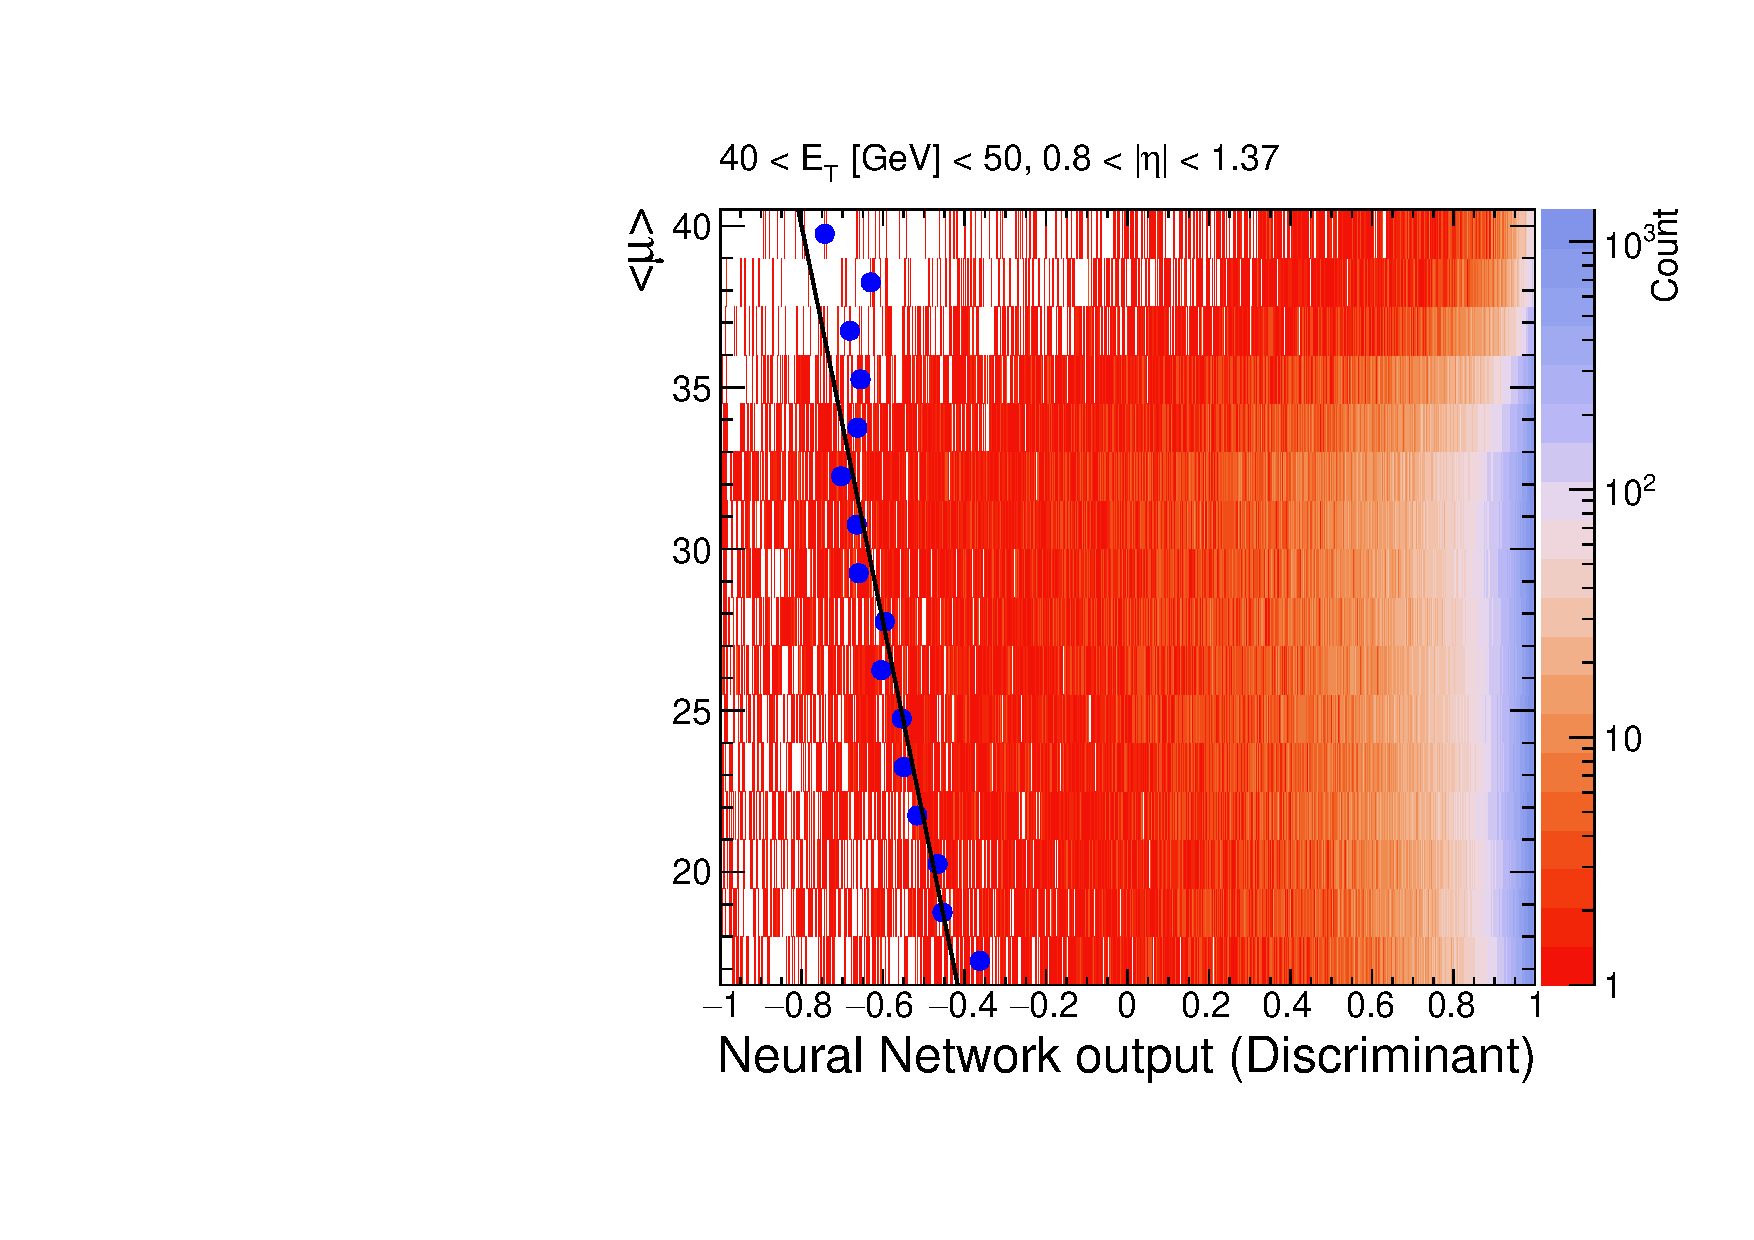
\includegraphics[width=\textwidth]{sections/ringer/figures/th2_signal_tight_cutbased_et3_eta1_with_tansig.pdf}
  \caption{Neural output with hyperbolic tangent w.r.t pileup.}
  \label{fig:nn_correction_with_tansig}
  \end{subfigure}
  \hfill
  \begin{subfigure}[c]{.48\textwidth}
  \centering
  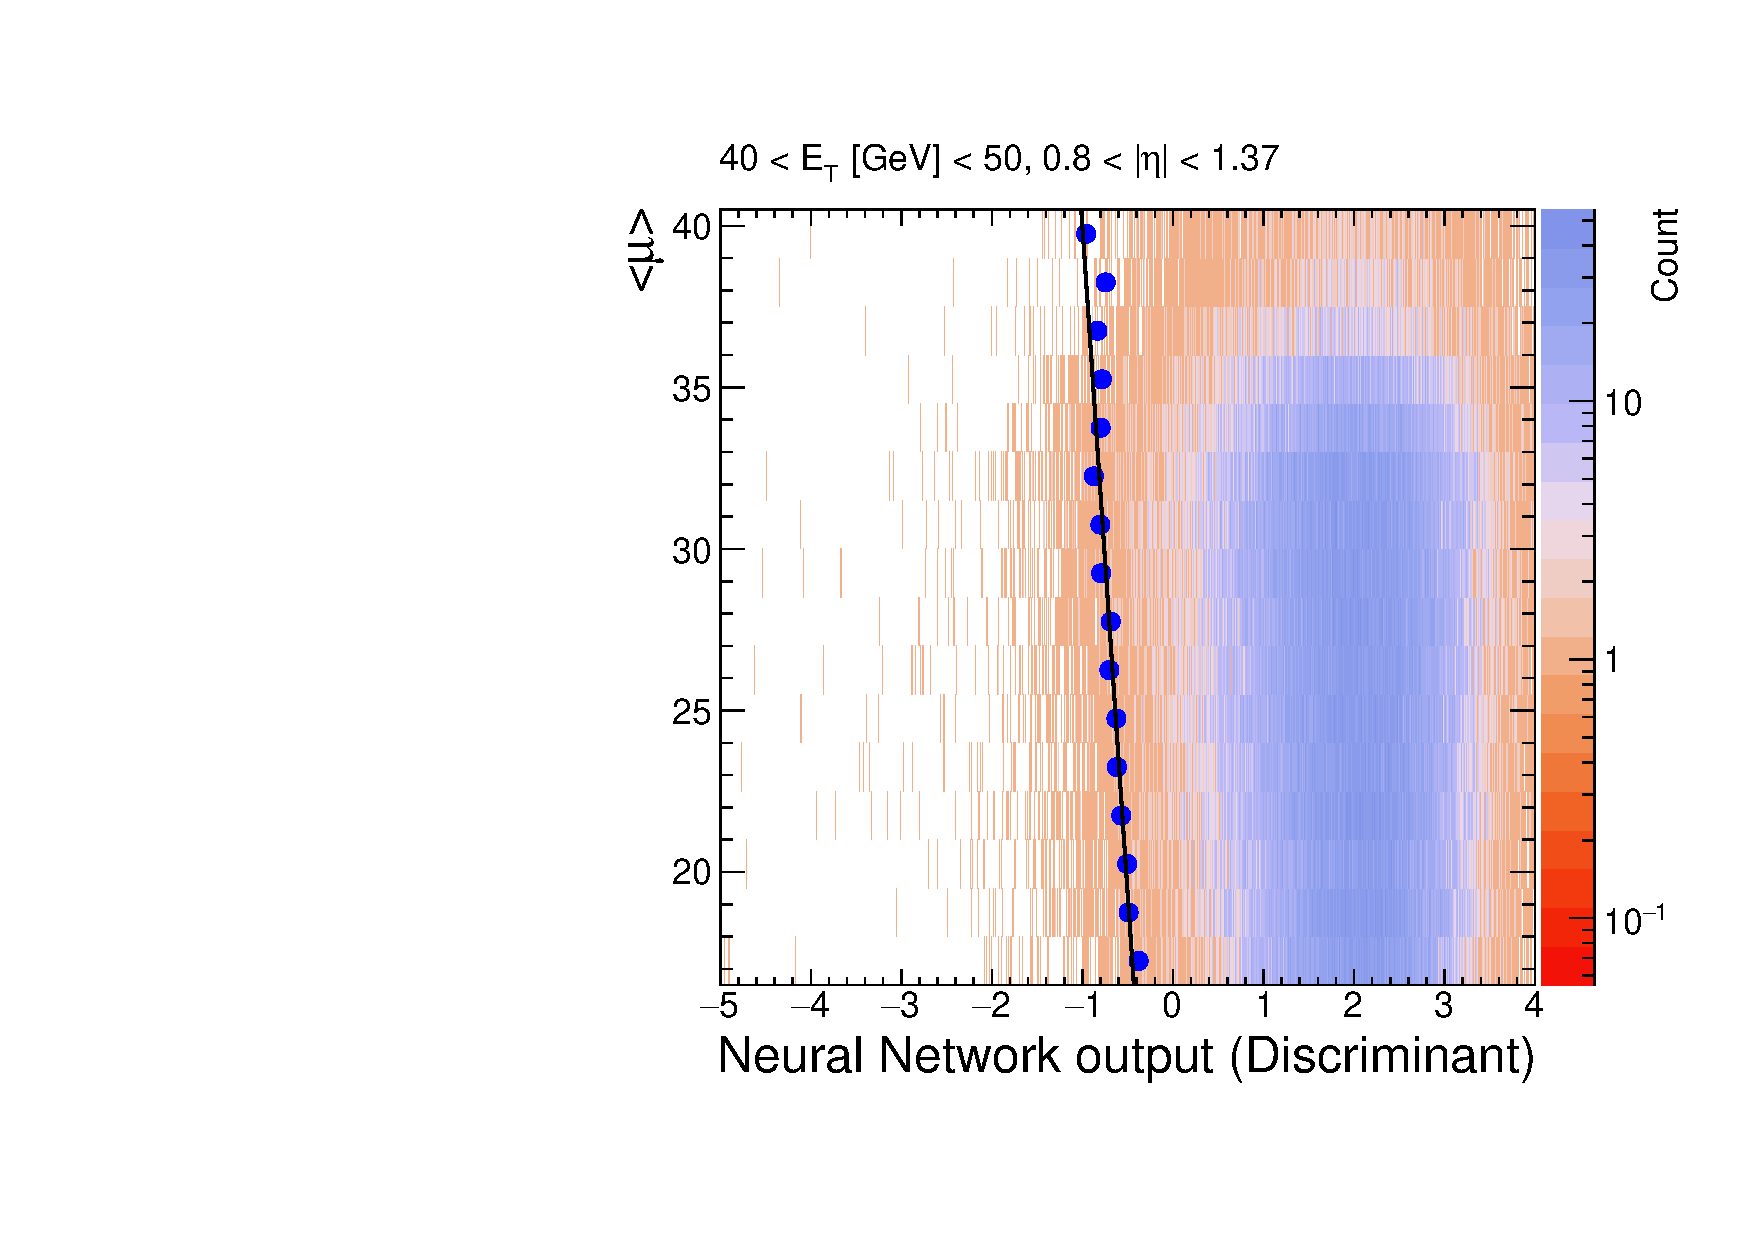
\includegraphics[width=\textwidth]{sections/ringer/figures/th2_signal_tight_cutbased_et3_eta1_without_tansig.pdf}
  \caption{Neural output with linear activation w.r.t pileup.}
  \label{fig:nn_correction_without_tansig}
  \end{subfigure}
  %\hfill
  \caption{
    \rnn output as a function of \avgmu{} for $Z\rightarrow ee$ probes in 
    2016 collision data.
    The computed threshold per \avgmu{} unit for achieving the target 
    efficiency is shown in blue full circle. The black line is a linear fit of the thresholds.
    The output space is computed using the trained model without modifications 
    in (a), while in (b) the output activation is replaced by the identity.
    The electron probes are selected using the training criteria.
  }%
  \end{center}
  \end{figure}




%
\begin{table*}[htb]
\caption{Boundaries in absolute electron pseudorapidity used to define the bins
  of the ensemble. The term `MLP' refers to the boundaries for the operation of
  the \rnn{} specialist network and with the `discriminant' term we define the
  boundaries for defining the thresholds for each requirement. Here, \emph{both}
refers to the computation of either the model parameters or the discriminant
respecting the same boundaries.}%
\label{tab:comp_etabins}
\begin{center}
\begin{tabular}{lcccccc}
\hline
\multicolumn{7}{c}{2017 \rnn  bin boundaries in \abseta}\\
\hline
MLP & 0.0 & 0.8& 1.37& 1.54& & 2.5 \\
Discriminant & 0.0& 0.8& 1.37& 1.54& 2.37 & 2.5 \\
\hline
\multicolumn{7}{c}{2018 \rnn  bin boundaries in \abseta}\\
\hline
Both & 0.0 & 0.8& 1.37& 1.52& 2.37 & 2.47 \\
\hline
\end{tabular}
\end{center}
\end{table*}



%


\begin{table*}[htb]
\caption{Boundaries in electron transverse energy defining the specialist
  network and discriminant threshold values to be employed by the \rnn{}
  algorithm.
}%
\label{tab:comp_etbins}
\begin{center}
\begin{tabular}{cccccc}
\hline
\multicolumn{6}{c}{2017 and 2018 \rnn bin boundaries in \Et [\GeV]}\\
\hline
15& 20& 30& 40& 50 & $\infty$ \\
\hline
\end{tabular}
\end{center}
\end{table*}






% TODO A plot showing the particular impact in the 2.37 region
% TODO Cross-validation: error bars
% TODO MLP training example
\begin{figure}[h!t]
\centering
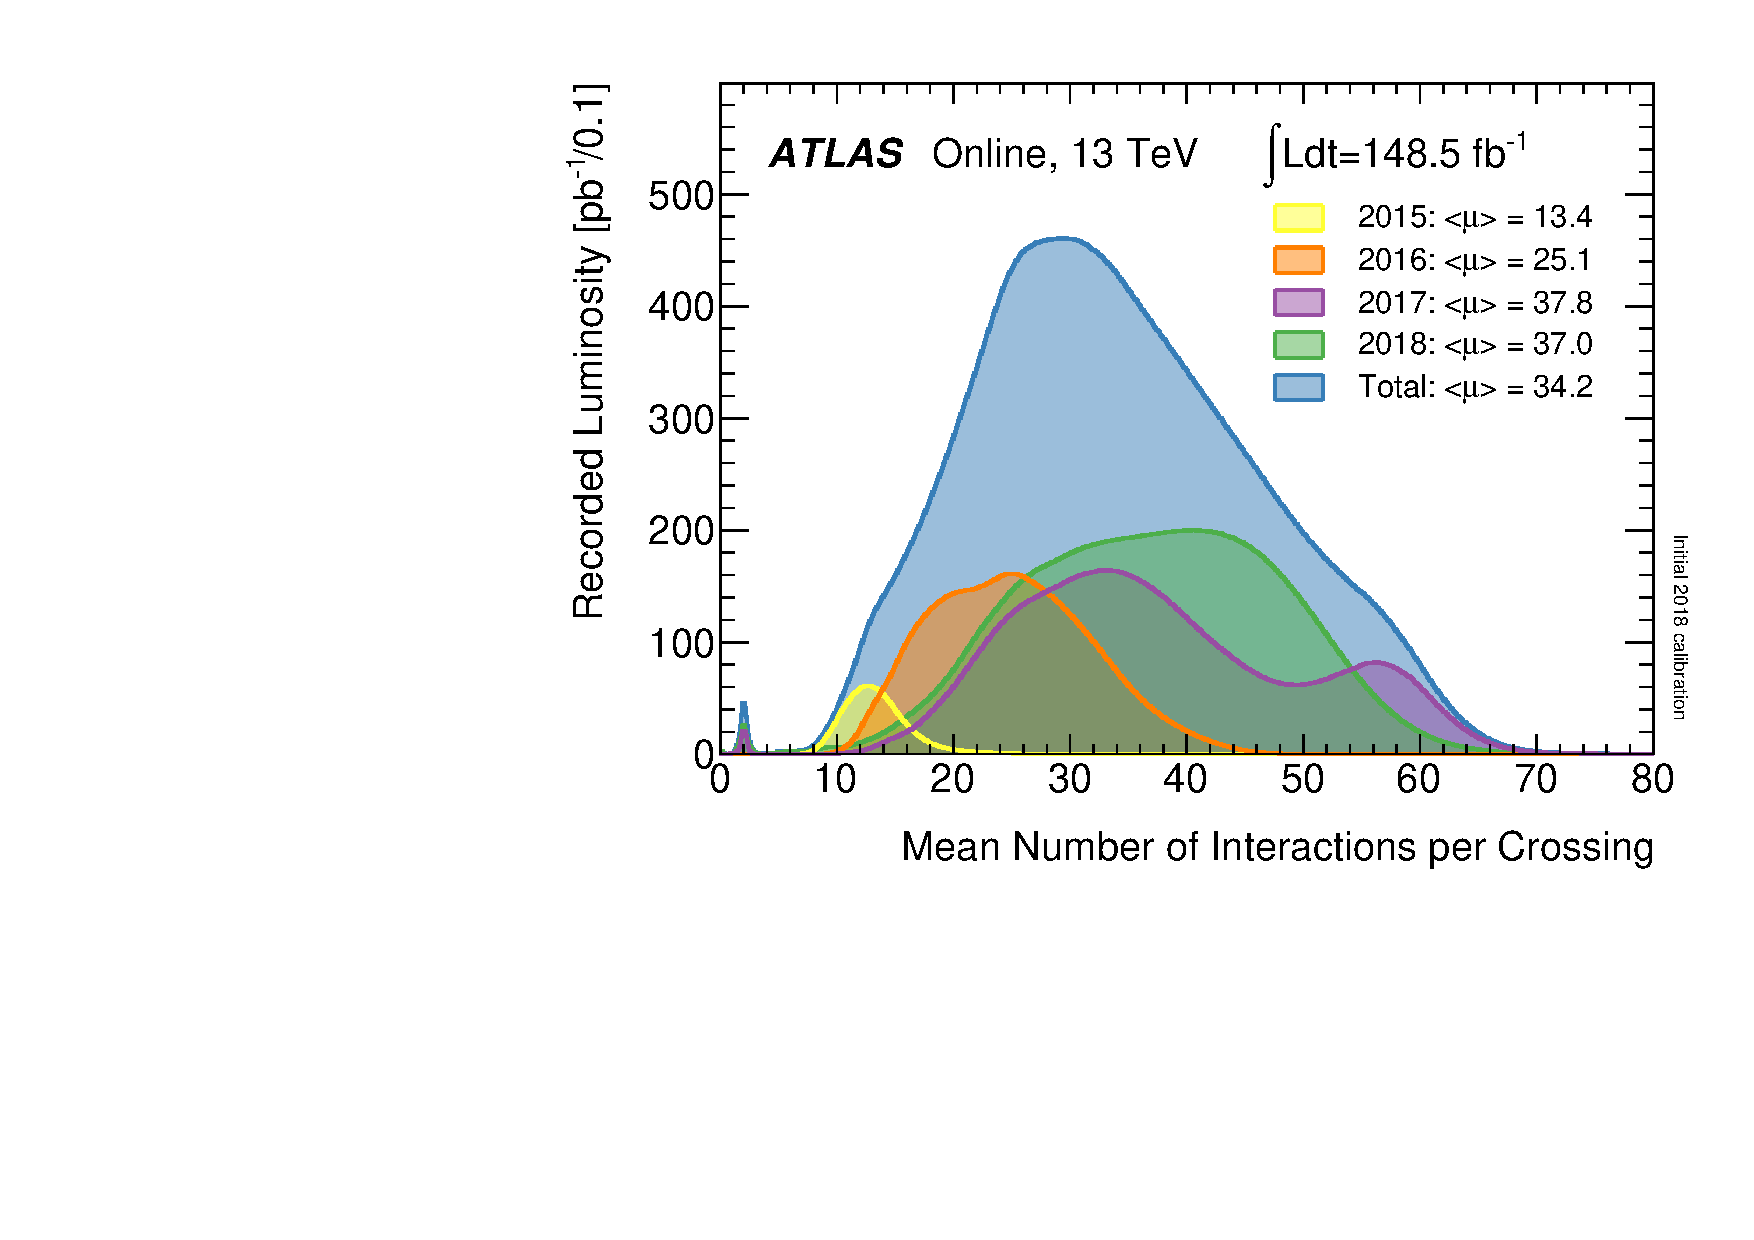
\includegraphics[width=0.6\textwidth]{sections/ringer/figures/mu_2015_2018.pdf}
\caption{\label{fig:mu_2015_2018}
Luminosity-weighted distribution of the mean number of interactions per crossing
for the Run~2 pp collision data at 13 TeV centre-of-mass
energy.~\cite{atlas_lumi_run2_results}}
\end{figure}


The linear correction applied during 2017 is upper-bounded by $\avgmu=40$
collisions, a quantile encompassing a large fraction of 2016 data
(Figure~\ref{fig:mu_2015_2018}). The objective was to avoid extrapolation to a
regime not previously evaluated, which could lead to unexpected growth in the
background rate and, thus, to data-taking issues due to the large CPU demand
from the electron triggers.

% (decision taking)
To account for Monte Carlo data mis-modeling, the parameters of the linear threshold
correction were derived using 2016 collision data. Furthermore, it was observed
that the rings in the region $2.37<\abseta<2.47$ had particular profiles due to
the lack of strip cells in this region and demanded a specific discriminant requirement in order to keep signal efficiencies near triggers without the \rnn{}. In order to avoid retraining all models, it was decided to split the last $|\eta|$ region in two ($1.37\rightarrow 2.5$ to $1.37\rightarrow2.37\rightarrow2.5$) and duplicate all models, for this region, to the new bin. Finally, the ensemble used to operates in 2017 has a total of 25 MLP models.



%It drastically affected the ring profiles in this region which resulted in a shift
%of the signal discriminant towards the direction of the background target and
%demanded a specific discriminant requirement in order to keep signal
%efficiencies near triggers without \rnn{}.

\FloatBarrier
\subsection{Training Procedure For 2018 Data}\label{ssec:2018}

Most of the procedure was kept unchanged for 2018, with modifications shown in
Table~\ref{tab:2018_ringer}.
In opposition to 2017, the developments for 2018
could benefit from collision data 
representing similar data taking conditions.
%In 2018, the developments could benefit from collision data representing similar conditions to data taking. 
The major alteration in 2018 tunes was the derivation of the \rnn{} ensemble with collision data based on \Zee{} \tnp{} event selection, in order to avoid the Monte Carlo data mis-modeling.

We also simplified the training strategy by abandoning the selection of three
models for each training and keeping only the \spmax{} model as the previous approach was more complex without a clear
payoff in trigger efficiency.
Likewise, MLPs with 5 to 10 units in the (single) hidden layer were tuned, as most models did not require
more than 10 units in 2017. With a larger time span for entering operation, we
added MLPs specialized in the region where we detected a change in the ring
profiles before 2017 operation ($2.37<\abseta<2.47$), resulting in the operation of
\SI{25}{MLPs}. The correction limit was set to
$\avgmu{}=100$~collisions or, in other words, removed for 2018 operation, given
that the data-taking 
conditions never reached such a large pileup level. By
%conditions did not extrapolate this value. By 
assuming a linear efficiency extrapolation,%\footnote{It is worth noticing that the linear
%fit is reasonably good for the Run~2 conditions.}
it was observed that most phase space regions did not reach background efficiencies
larger than \SI{15}{\%} before arriving at $\avgmu=100$~collisions, while same
signal efficiencies were maintained.

% NOTE TriggerEgammaMeeting_20180213

% NOTE TriggerEgammaMeeting_20180213

\begin{table}[ht!]\footnotesize
\centering
\caption{Changes in the derivation of the 2018 \rnn operation models with
respect to 2017 models. See text for more details.}\label{tab:2018_ringer}
\resizebox{\textwidth}{!}{%
\begin{tabular}{p{6cm}p{10cm}}
\hline
\hline
\hline
Criterion & Value \\
\hline
\hline
\multicolumn{2}{c}{Ensemble Composition} \\
\hline
\hline
Phase space bins for Model Tuning &
Added one new boundary for the tunes in \eta, see Table~\ref{tab:ensemble_regions} \\
\\
\hline
\hline
\multicolumn{2}{c}{MLP Training} \\
\hline
\hline

Dataset and event selection & 2017 $13$ TeV $p-p$ collision data (Section~\ref{ssec:dataset})
\\ 
Over-training evaluation & Stop when fail to improve \spmax for 50 epochs
(compute ROC at each epoch) \\

Evaluated topologies & Hidden layer with number of neurons ranging from 5 to 10
units \\

\hline
\hline
\multicolumn{2}{c}{Training Evaluation and Selection of the Operating Model} \\
\hline
\hline

\multicolumn{2}{c}{All criteria with same configuration} \\

\hline
\hline
\multicolumn{2}{c}{Decision Making} \\
\hline
\hline

Fit Method & Linear fit method
$\chi^2=\frac{{(y-f(x))}^2}{e_y^2+{(0,5{(e_{xl}+e_{xh})}f\prime(x))}^2}$ 
where $f(x)$ is the function to be fitted, in this case an affine function; and $y$ is the lower (upper) error of the ordinates if $f(x)$ is below (above) $y$, and $e_{xl}$ ($e_{xh}$) is the lower (upper) error on the abscissas. \\
Dataset and event selection & 2017 $13\;\text{TeV}$ p-p collision data (GRL:
v97), except for reprocessing reference run \\

Decision Making Strategy & Linear fit of the network output by replacing the transfer function w.r.t. $\avgmu$ up to 100$\;$avg.\@ collisions.
When $\avgmu >100$, set $\avgmu = 100$ \\

\hline
\hline
\hline
\end{tabular}
}
\end{table}







